\documentclass[tikz,border=4pt]{standalone}
\usepackage[T1]{fontenc}
\usepackage{lmodern,amssymb,amsmath}
% stile comune delle figure "da brevetto": bianco e nero, linee sottili, numeri di riferimento
\usetikzlibrary{arrows.meta,calc,patterns,decorations.pathmorphing,decorations.pathreplacing,positioning}
\tikzset{
  every node/.style={font=\scriptsize},
  arr/.style={-{Latex[length=1.8mm,width=1.3mm]}, line width=0.55pt},
  darr/.style={arr, dashed},
  blk/.style={draw, line width=0.6pt, align=center, font=\scriptsize, inner sep=2.5pt},
  thinl/.style={line width=0.35pt},
  figlab/.style={font=\large\bfseries},
}
% \leader{punto}{posizione del numero}{anchor}{numero}
\newcommand{\leader}[4]{\draw[line width=0.3pt] (#1) to[bend left=12] (#2) node[anchor=#3, inner sep=1pt, font=\small]{#4};}

\begin{document}
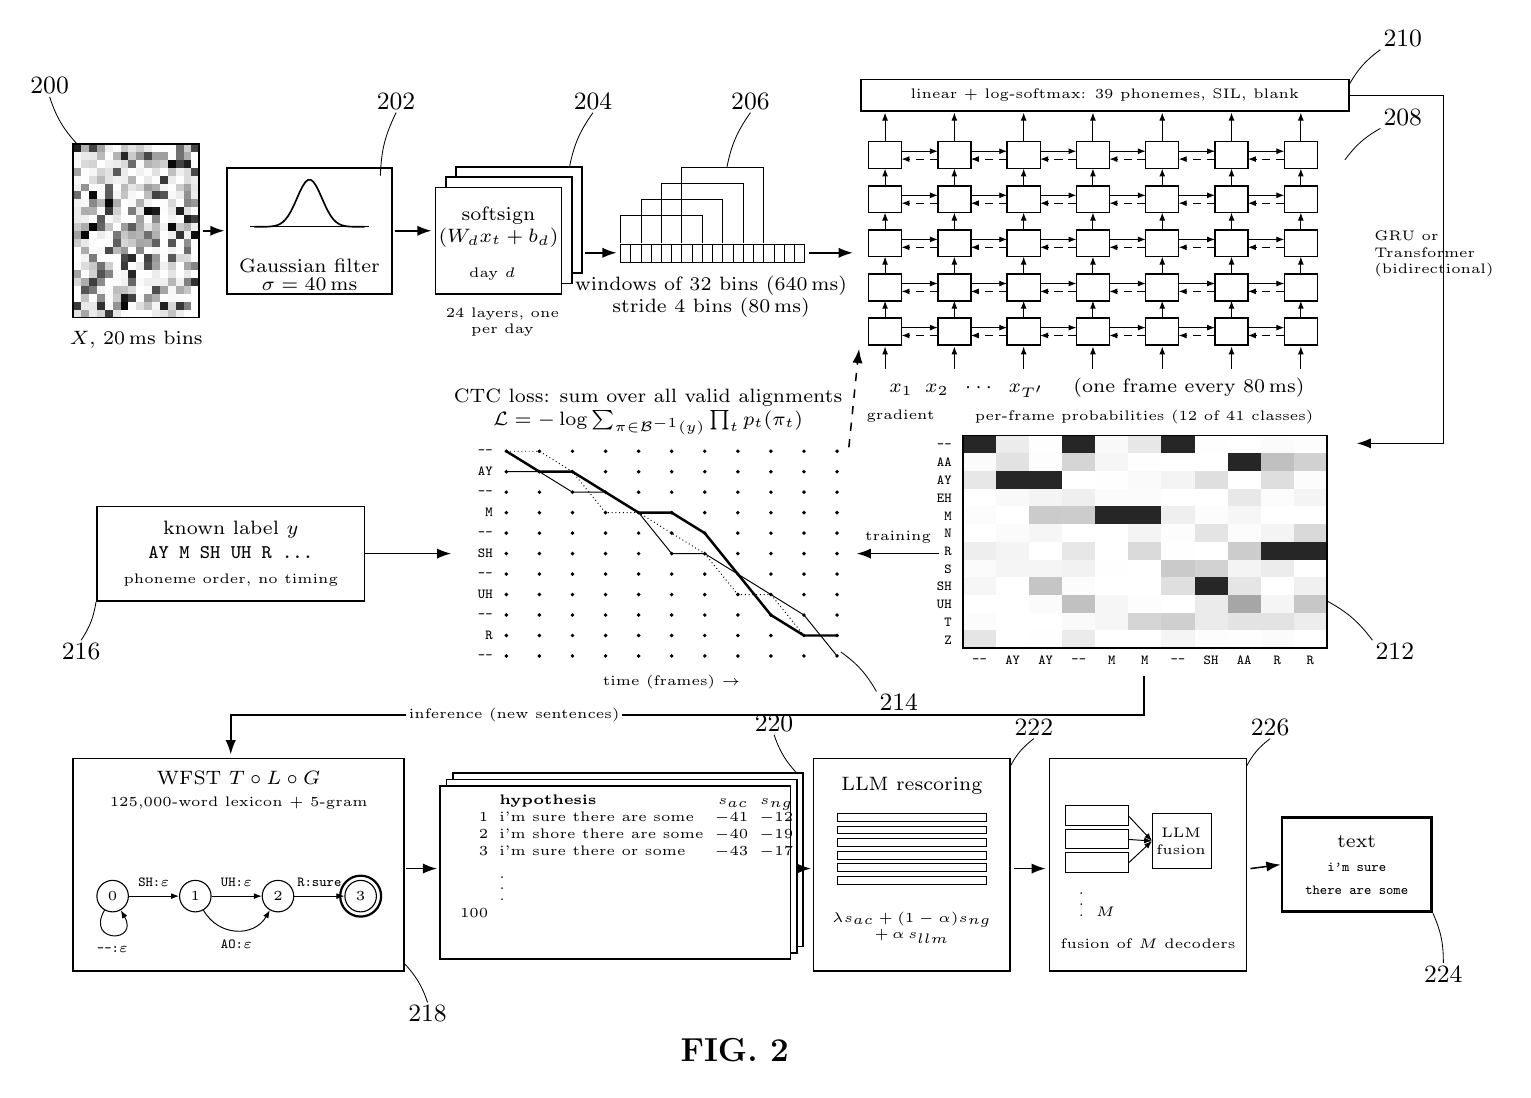
\begin{tikzpicture}[x=1cm,y=1cm]
\pgfmathsetseed{5}

% ================= riga A: pre-elaborazione e rete =================
% 200: matrice X
\begin{scope}[shift={(0,8.6)}]
\foreach \i in {0,...,15} \foreach \j in {0,...,21} {
  \pgfmathsetmacro{\g}{100*rnd^3}
  \fill[black!\g] (\i*0.1,\j*0.1) rectangle ++(0.1,0.1);}
\draw[line width=0.6pt] (0,0) rectangle (1.6,2.2);
\end{scope}
\node[anchor=north] at (0.8,8.55) {$X$, 20\,ms bins};
\leader{0.05,10.8}{-0.3,11.4}{south}{200}

% 202: filtro gaussiano
\draw[line width=0.6pt] (1.95,8.9) rectangle (4.05,10.5);
\draw[thinl] (2.25,9.75) -- (3.75,9.75);
\draw[line width=0.6pt] plot[domain=-0.7:0.7, samples=40] ({3.0+\x},{9.75+0.6*exp(-\x*\x/0.05)});
\node at (3.0,9.25) {Gaussian filter};
\node at (3.0,9.02) {$\sigma=40$\,ms};
\draw[arr] (1.65,9.7) -- (1.92,9.7);
\leader{3.9,10.4}{4.1,11.2}{south}{202}

% 204: strato per giorno
\foreach \k in {2,1,0} \draw[line width=0.6pt, fill=white] (4.6+\k*0.13,8.9+\k*0.13) rectangle ++(1.6,1.35);
\node[align=center] at (5.4,9.75) {$\mathrm{softsign}$\\$(W_d x_t + b_d)$};
\node[align=center, font=\tiny] at (5.32,9.15) {day $d$};
\node[anchor=north, align=center, font=\tiny] at (5.45,8.85) {24 layers, one\\per day};
\draw[arr] (4.08,9.7) -- (4.55,9.7);
\leader{6.3,10.5}{6.6,11.2}{south}{204}

% 206: finestre temporali
\foreach \b in {0,...,17} \draw[thinl] (6.95+\b*0.13,9.3) rectangle ++(0.13,0.22);
\foreach \w/\h in {0/0.35,2/0.55,4/0.75,6/0.95} {
  \draw[thinl] (6.95+\w*0.13,9.55) -- ++(0,\h) -- ++(1.04,0) -- ++(0,-\h);}
\node[align=center, anchor=north] at (8.1,9.25) {windows of 32 bins (640\,ms)\\stride 4 bins (80\,ms)};
\draw[arr] (6.5,9.42) -- (6.9,9.42);
\leader{8.3,10.5}{8.6,11.2}{south}{206}
\draw[arr] (9.35,9.42) -- (9.9,9.42);

% 208: rete ricorrente srotolata nel tempo (5 strati x 7 passi)
\foreach \l in {0,...,4} \foreach \t in {0,...,6} {
  \draw[line width=0.5pt, fill=white] (10.1+\t*0.88,8.25+\l*0.56) rectangle ++(0.42,0.34);}
\foreach \l in {0,...,4} \foreach \t in {0,...,5} {
  \draw[-{Latex[length=1mm]}, line width=0.35pt] (10.52+\t*0.88,8.47+\l*0.56) -- ++(0.46,0);
  \draw[-{Latex[length=1mm]}, line width=0.3pt, densely dashed] (10.98+\t*0.88,8.37+\l*0.56) -- ++(-0.46,0);}
\foreach \l in {0,...,3} \foreach \t in {0,...,6} \draw[-{Latex[length=1mm]}, line width=0.35pt] (10.31+\t*0.88,8.59+\l*0.56) -- ++(0,0.22);
\foreach \t in {0,...,6} {
  \draw[-{Latex[length=1mm]}, line width=0.35pt] (10.31+\t*0.88,7.95) -- ++(0,0.28);
  \draw[-{Latex[length=1mm]}, line width=0.35pt] (10.31+\t*0.88,10.84) -- ++(0,0.36);}
\node[anchor=north] at (13.0,7.95) {$x_1 \;\; x_2 \;\; \cdots \;\; x_{T'}$ \quad (one frame every 80\,ms)};
\node[anchor=west, align=left, font=\tiny] at (16.4,9.4) {GRU or\\Transformer\\(bidirectional)};
\leader{16.15,10.6}{16.6,11.0}{south west}{208}

% 210: testa lineare
\draw[line width=0.6pt] (10.0,11.22) rectangle (16.2,11.62);
\node[font=\tiny] at (13.1,11.42) {linear + log-softmax: 39 phonemes, SIL, blank};
\leader{16.2,11.55}{16.6,12.0}{south west}{210}
\draw[arr] (16.2,11.42) -- (17.4,11.42) -- (17.4,7.0) -- (16.3,7.0);

% ================= riga B: posteriori e CTC =================
% 212: posteriorgramma (12 classi mostrate su 41, 11 frame)
\def\seq{0,1,1,0,2,2,0,3,4,5,5}
\def\cls{{"--","AY","M","SH","AA","R"}}
\begin{scope}[shift={(11.3,4.4)}]
\foreach \c [count=\r from 0] in {--,AA,AY,EH,M,N,R,S,SH,UH,T,Z} \node[anchor=east, font=\tiny\ttfamily] at (-0.02,2.7-\r*0.225-0.12) {\c};
\foreach \t in {0,...,10} \foreach \r in {0,...,11} {
  \pgfmathsetmacro{\g}{25*rnd^4}
  \fill[black!\g] (\t*0.42,2.7-\r*0.225) rectangle ++(0.42,-0.225);}
% celle dominanti: righe 0=--,2=AY,4=M,8=SH,1=AA,6=R
\foreach \t/\r in {0/0,1/2,2/2,3/0,4/4,5/4,6/0,7/8,8/1,9/6,10/6}
  \fill[black!85] (\t*0.42,2.7-\r*0.225) rectangle ++(0.42,-0.225);
\fill[black!35] (8*0.42,2.7-9*0.225) rectangle ++(0.42,-0.225);
\draw[line width=0.6pt] (0,0) rectangle (4.62,2.7);
\foreach \t/\s in {0/--,1/AY,2/AY,3/--,4/M,5/M,6/--,7/SH,8/AA,9/R,10/R}
  \node[font=\tiny\ttfamily] at (\t*0.42+0.21,-0.15) {\s};
\end{scope}
\node[anchor=south, align=center, font=\tiny] at (13.6,7.12) {per-frame probabilities (12 of 41 classes)};
\leader{15.92,5.0}{16.5,4.5}{north west}{212}

% 214: traliccio CTC (addestramento)
\begin{scope}[shift={(5.5,4.3)}]
\def\lab{{"--","AY","--","M","--","SH","--","UH","--","R","--"}}
\foreach \s in {0,...,10} {
  \pgfmathsetmacro{\name}{\lab[\s]}
  \node[anchor=east, font=\tiny\ttfamily] at (-0.05,2.6-\s*0.26) {\name};
  \foreach \t in {0,...,10} \fill (\t*0.42,2.6-\s*0.26) circle (0.025);}
% percorsi validi: uno in grassetto, due sottili
\draw[line width=0.9pt] (0,2.6) -- (0.42,2.34) -- (0.84,2.34) -- (1.26,2.08) -- (1.68,1.82) -- (2.1,1.82) -- (2.52,1.56) -- (2.94,1.04) -- (3.36,0.52) -- (3.78,0.26) -- (4.2,0.26);
\draw[line width=0.35pt] (0,2.34) -- (0.42,2.34) -- (0.84,2.08) -- (1.26,2.08) -- (1.68,1.82) -- (2.1,1.3) -- (2.52,1.3) -- (2.94,1.04) -- (3.36,0.78) -- (3.78,0.52) -- (4.2,0);
\draw[line width=0.35pt, densely dotted] (0,2.6) -- (0.42,2.6) -- (0.84,2.34) -- (1.26,1.82) -- (1.68,1.82) -- (2.1,1.56) -- (2.52,1.3) -- (2.94,0.78) -- (3.36,0.78) -- (3.78,0.26) -- (4.2,0.26);
\node[anchor=north, font=\tiny] at (2.1,-0.12) {time (frames) $\rightarrow$};
\end{scope}
\node[anchor=south, align=center] at (7.3,6.98) {CTC loss: sum over all valid alignments\\$\mathcal{L}=-\log\sum_{\pi\in\mathcal{B}^{-1}(y)}\prod_t p_t(\pi_t)$};
\leader{9.75,4.35}{10.2,3.85}{north west}{214}
\draw[arr] (11.0,5.6) -- node[above, font=\tiny] {training} (9.95,5.6);

% 216: etichetta y
\node[blk, minimum width=3.4cm, minimum height=1.2cm, align=center] (y) at (2.0,5.6) {known label $y$\\[1pt]\texttt{AY M SH UH R ...}\\[1pt]{\tiny phoneme order, no timing}};
\draw[arr] (y.east) -- (4.8,5.6);
\leader{y.south west}{0.1,4.5}{north}{216}
% gradiente verso la rete
\draw[darr] (9.85,6.95) .. controls (9.9,7.5) .. (9.98,8.2);
\node[font=\tiny, anchor=west] at (9.95,7.35) {gradient};

% ================= riga C: decodifica con modelli linguistici =================
\draw[arr] (13.6,4.05) -- (13.6,3.55) -- (2.0,3.55) -- (2.0,3.05);
\node[fill=white, inner sep=1pt, font=\tiny] at (5.6,3.55) {inference (new sentences)};

% 218: WFST
\draw[line width=0.6pt] (0,0.3) rectangle (4.2,3.0);
\node[align=center] at (2.1,2.6) {WFST $T\circ L\circ G$\\{\tiny 125,000-word lexicon + 5-gram}};
\foreach \n/\x in {0/0.5,1/1.55,2/2.6,3/3.65} \node[draw, circle, inner sep=0pt, minimum size=4mm, font=\tiny] (q\n) at (\x,1.25) {\n};
\draw[line width=0.8pt] (q3) circle (2.6mm);
\draw[-{Latex[length=1mm]}, thinl] (q0) -- node[above, font=\tiny\ttfamily] {SH:$\varepsilon$} (q1);
\draw[-{Latex[length=1mm]}, thinl] (q1) -- node[above, font=\tiny\ttfamily] {UH:$\varepsilon$} (q2);
\draw[-{Latex[length=1mm]}, thinl] (q2) -- node[above, font=\tiny\ttfamily] {R:sure} (q3);
\draw[-{Latex[length=1mm]}, thinl] (q0) to[out=240,in=300,looseness=6] node[below, font=\tiny\ttfamily] {--:$\varepsilon$} (q0);
\draw[-{Latex[length=1mm]}, thinl] (q1) to[out=-60,in=-120,looseness=1.2] node[below, font=\tiny\ttfamily] {AO:$\varepsilon$} (q2);
\leader{4.2,0.4}{4.5,-0.1}{north}{218}

% 220: lista delle 100 ipotesi
\foreach \k in {2,1,0} \draw[line width=0.6pt, fill=white] (4.66+\k*0.08,0.45+\k*0.08) rectangle ++(4.45,2.2);
\node[anchor=north west, font=\tiny, inner sep=1pt] at (4.8,2.6) {%
\setlength{\tabcolsep}{2pt}\begin{tabular}{rlrr}
& \textbf{hypothesis} & $s_{ac}$ & $s_{ng}$\\
1 & i'm sure there are some & $-$41 & $-$12\\
2 & i'm shore there are some & $-$40 & $-$19\\
3 & i'm sure there or some & $-$43 & $-$17\\
 & $\vdots$ & & \\
100 & & & \end{tabular}};
\draw[arr] (4.22,1.6) -- (4.62,1.6);
\leader{9.2,2.8}{8.9,3.3}{south}{220}

% 222: LLM
\draw[line width=0.6pt] (9.4,0.3) rectangle (11.9,3.0);
\foreach \k in {0,...,5} \draw[thinl] (9.7,1.4+\k*0.16) rectangle (11.6,1.5+\k*0.16);
\node[align=center] at (10.65,2.65) {LLM rescoring};
\node[align=center, font=\tiny] at (10.65,0.85) {$\lambda s_{ac}+(1-\alpha)s_{ng}$\\$+\,\alpha\, s_{llm}$};
\draw[arr] (9.28,1.6) -- (9.37,1.6);
\leader{11.9,2.9}{12.2,3.25}{south}{222}

% 226: ensemble (in sviluppo)
\draw[line width=0.6pt] (12.4,0.3) rectangle (14.9,3.0);
\foreach \k in {0,1,2} \draw[thinl] (12.6,2.15-\k*0.3) rectangle (13.4,2.4-\k*0.3);
\node[font=\tiny] at (13.0,1.25) {$\vdots$ \;$M$};
\foreach \k in {0,1,2} \draw[-{Latex[length=1mm]}, thinl] (13.4,2.27-\k*0.3) -- (13.7,1.95);
\draw[thinl] (13.7,1.6) rectangle (14.45,2.3);
\node[font=\tiny, align=center] at (14.07,1.95) {LLM\\fusion};
\node[font=\tiny, align=center] at (13.65,0.65) {fusion of $M$ decoders};
\draw[arr] (11.95,1.6) -- (12.35,1.6);
\leader{14.9,2.9}{15.2,3.25}{south}{226}

% 224: testo
\node[blk, minimum width=1.9cm, minimum height=1.2cm, line width=1pt] (out) at (16.3,1.65) {text\\[1pt]\texttt{\tiny i'm sure}\\\texttt{\tiny there are some}};
\draw[arr] (14.95,1.6) -- (out.west);
\leader{out.south east}{17.4,0.4}{north}{224}

\node[figlab] at (8.4,-0.7) {FIG. 2};
\end{tikzpicture}
\end{document}
